\documentclass[a4paper, 11pt]{article}

% Pacotes Essenciais ========================================================================
\usepackage[utf8]{inputenc}
\usepackage[brazilian]{babel}
\usepackage[T1]{fontenc}
\usepackage{graphicx}
\usepackage[svgnames,table]{xcolor}
\usepackage{subcaption}
\usepackage[lmargin=2.5cm,tmargin=4cm,rmargin=2cm,bmargin=3.5cm,headheight=15.1pt]{geometry}
\usepackage[onehalfspacing]{setspace}
\usepackage{indentfirst}
\usepackage{enumerate}
\usepackage{nameref}
\usepackage{anyfontsize}
\usepackage{blindtext,lipsum,comment}
\usepackage{multicol,multirow}
\usepackage[hidelinks]{hyperref}
\usepackage{titlesec}

% Tabelas e Alinhamento =====================================================================
\usepackage{booktabs} % <--- ADICIONADO PARA RESOLVER O ERRO DA TABELA
\usepackage{tabularx}
\usepackage{longtable}
\usepackage{float}
\usepackage{array}
\usepackage{adjustbox}
\usepackage{ragged2e}

% TikZ e Gráficos ===========================================================================
\usepackage{tikz}
\usetikzlibrary{calc,patterns,arrows}
\usepackage{pgfplots}
\pgfplotsset{compat=1.17}
\usepgfplotslibrary{fillbetween}

% Estética e Fontes =========================================================================
\usepackage{fancyhdr}
\usepackage{calligra}
\usepackage{helvet}
\usepackage{pifont}
\usepackage{datetime}
\usepackage{lastpage}
\usepackage[font=sf,labelfont=bf]{caption}

\definecolor{cinza}{HTML}{595959}
\definecolor{verdeEJ}{HTML}{92D050}
\newcolumntype{g}{>{\columncolor[HTML]{92D050}} c }

\renewcommand{\headrulewidth}{0pt}
\renewcommand{\footrulewidth}{0pt}

\pagestyle{fancy}
\cfoot{{\color{cinza}
\footnotesize{\fontfamily{phv}\selectfont
\textbf{
Brasília, \today. \\
ELETRONJUN – UNIVERSIDADE DE BRASÍLIA \\
EMPRESA JÚNIOR DE ENGENHARIA ELETRÔNICA\\}
Área Especial de Indústria – Projeção A| 72444-240 | Gama/DF \\
www.eletronjun.com.br | contato@eletronjun.com.br}}
}

% Bibliografia e Citações ===================================================================
\usepackage[alf,abnt-repeated-title-omit=yes,abnt-emphasize=bf,abnt-etal-list=0]{abntex2cite}
\citebrackets()

% Matemática ================================================================================
\usepackage{amsfonts,amssymb,amsthm,amsmath,dsfont,mathtools}
\everymath{\displaystyle}
\newcommand{\pra}{\ding{118}}
\newcommand{\NN}{\mathds{N}}
\newcommand{\ZZ}{\mathds{Z}}
\newcommand{\QQ}{\mathds{Q}}
\newcommand{\RR}{\mathds{R}}
\newcommand{\CC}{\mathds{C}}

% Códigos (Listings) ========================================================================
\usepackage{listings}
\definecolor{codegreen}{rgb}{0,0.6,0}
\definecolor{codegray}{rgb}{0.5,0.5,0.5}
\definecolor{codepurple}{rgb}{0.58,0,0.82}
\definecolor{backcolour}{rgb}{0.95,0.95,0.92}

\lstdefinestyle{mystyle}{
    backgroundcolor=\color{backcolour},   
    commentstyle=\color{codegreen},
    keywordstyle=\color{magenta},
    numberstyle=\tiny\color{codegray},
    stringstyle=\color{codepurple},
    basicstyle=\ttfamily\footnotesize,
    breaklines=true,                 
    captionpos=b,                    
    numbers=left,                    
    numbersep=5pt,                  
    tabsize=2
}
\lstset{style=mystyle}
\renewcommand\lstlistingname{Algoritmo}

% Ambientes Personalizados (Requisitos) =====================================================
\usepackage{enumitem}
\newcounter{rfreq}
\newenvironment{rfreq}[1]{
    \refstepcounter{rfreq}
    \subsubsection{[RF\ifnum\value{rfreq}<10 0\fi\arabic{rfreq}] \textcolor{black}{[#1]}}
    \begin{flushright}\begin{minipage}{0.9\textwidth}
}{
    \end{minipage}\end{flushright}
}

\newcounter{nfreq}
\newenvironment{nfreq}[1]{
    \refstepcounter{nfreq}
    \subsubsection{[NF\ifnum\value{nfreq}<10 0\fi\arabic{nfreq}] \textcolor{black}{[#1]}}
    \begin{flushright}\begin{minipage}{0.9\textwidth}
}{
    \end{minipage}\end{flushright}
}

\titleformat*{\section}{\color{verdeEJ}\Large\fontfamily{phv}\selectfont\bfseries}
\titleformat*{\subsection}{\color{verdeEJ}\large\fontfamily{phv}\selectfont\bfseries}
\titleformat*{\subsubsection}{\color{verdeEJ}\large\fontfamily{phv}\selectfont}

\begin{document}
\fontfamily{phv}\selectfont

\input{capa.tex} %%ALTERE A CAPA AQUI%%

\tableofcontents
\newpage
%%%%%%%%%%% EDITE A PARTIR DAQUI %%%%%%%%%% 
\section{Introdução}
O  projeto tem como objetivo o desenvolvimento de um sistema de monitoramento capaz de coletar dados de temperatura e umidade do ambiente e disponibilizá-los em tempo real por meio de uma interface web.

O sistema será composto por um sensor de temperatura e umidade, responsável pela aquisição dos dados ambientais, e por um microcontrolador, encarregado de processar essas informações, realizar a comunicação com a interface web e controlar os elementos de saída do sistema, como os LEDs indicadores de estado. A escolha desses componentes será fundamentada em critérios técnicos relevantes, como faixa de medição, precisão, consumo de energia, facilidade de integração e capacidade de comunicação em rede.

Além da aquisição e exibição dos dados, o sistema deverá permitir a interação com o usuário por meio de uma interface web, na qual será possível visualizar as medições em tempo real e alternar entre diferentes modos de operação. Os modos previstos são: desligado, no qual o sistema permanece inativo; automático, em que a coleta e exibição dos dados ocorrem de forma contínua; e ligado, no qual o sistema aguarda ações do usuário. A mudança de estado deverá ser refletida visualmente através de LEDs, proporcionando uma indicação clara e imediata do modo de operação atual.

O desenvolvimento do projeto envolve a integração entre hardware e software, implementando a lógica de funcionamento do sistema e da interface web. Dessa forma, busca-se construir uma solução funcional, organizada e alinhada aos requisitos propostos.


\newpage

\section{Análise de Requisitos}

A análise de requisitos é o levantamento de todas as propriedades, características e necessidades do sistema para que esse seja capaz de executar, com a qualidade desejada, as funcionalidades previstas. Essa seção serve de base tanto para o cliente, guiando as expectativas quanto ao projeto a partir da definição sólida de quais serão suas especificações, como para os projetistas, que, ao desenvolverem o sistema de acordo com os requisitos levantados, estarão seguros quanto à sua efetividade para o problema.

Os requisitos funcionais, dispostos na seção 2.2, são propriedades do sistema responsáveis por explicitar suas funcionalidades e como estas atendem às solicitações do projeto. A partir da leitura dos requisitos funcionais, tem-se noção do que o sistema deve ser capaz de executar e quais são as necessidades que ele busca suprir.

Os requisitos não-funcionais, dispostos na seção 2.3, são propriedades do sistema que mostram especificações e características relacionadas ao modo como os requisitos funcionais são operados. A partir da leitura dos requisitos não-funcionais, tem-se noção de informações técnicas e atributos de qualidade de execução das funcionalidades do sistema.

\subsection{Convenções, termos e abreviações}

\subsubsection{Identificação dos Requisitos}

Por convenção, a referência a requisitos é feita através do nome da subseção na qual eles
estão descritos, seguidos do identificador do requisito, de acordo com o seguinte modelo:
\begin{center}
    [ nome da subseção/identificador do requisito ]
\end{center}

Os requisitos serão identificados com um identificador único, com numeração iniciada em
[RF01] para um requisito funcional e [NF01] para um requisito não-funcional.

\subsubsection{Propriedades dos requisitos}

Para estabelecer a prioridade dos requisitos, nas seções 2.2 e 2.3, foram adotadas as
denominações “essencial”, “importante” e “desejável”, tal que:

\textbf{Essencial} é o requisito sem o qual o sistema não entra em funcionamento. Requisitos
essenciais são aqueles imprescindíveis, que devem ser implementados impreterivelmente.

\textbf{Importante} é o requisito sem o qual o sistema entra em funcionamento, mas de forma não
satisfatória. Requisitos importantes devem ser implementados, mas, se não forem, o sistema
poderá ser implementado e usado normalmente.

\textbf{Desejável} é o requisito que não compromete as funcionalidades básicas do sistema, isto é,
o sistema pode funcionar de forma satisfatória sem ele. Requisitos desejáveis podem ser deixados
para versões posteriores do sistema, caso não haja tempo hábil para implementação dos mesmos
nesta etapa.

\section{Análise de Requisitos}

\subsection{Requisitos Funcionais}

\begin{itemize}

\item \textbf{[RF01] (Essencial)} – O sistema deve coletar dados de temperatura e umidade do ambiente por meio de um sensor apropriado.

\item \textbf{[RF02] (Essencial)} – O sistema deve disponibilizar os dados coletados em uma interface web acessível ao usuário.

\item \textbf{[RF03] (Essencial)} – O sistema deve atualizar os dados de temperatura e umidade em tempo real na interface web.

\item \textbf{[RF04] (Essencial)} – O sistema deve permitir a alternância entre os modos de operação (Desligado, Automático e Ligado) através da interface web.

\item \textbf{[RF05] (Essencial)} – O sistema deve indicar visualmente o modo de operação atual por meio de LEDs no hardware.

\item \textbf{[RF06] (Essencial)} – O sistema deve sincronizar o estado dos LEDs com o modo selecionado na interface web.

\item \textbf{[RF07] (Essencial)} – No modo automático, o sistema deve realizar a coleta e atualização contínua dos dados.

\item \textbf{[RF08] (Essencial)} – No modo ligado, o sistema deve permanecer ativo e apto a responder às ações do usuário.

\item \textbf{[RF09] (Essencial)} – No modo desligado, o sistema deve interromper a coleta de dados e ativar o LED de desligado.

\item \textbf{[RF10] (Essencial)} – O sistema deve permitir a interface web atualizada sem necessidade de recarregamento manual da página.

\item \textbf{[RF11] (Essencial)} – No modo ligado, a interface deve disponibilizar botões para requisição manual de leitura de temperatura, umidade ou ambas.

\item \textbf{[RF12] (Importante)} – O sistema deve armazenar um histórico das leituras com data e hora, exibindo-o na interface web.

\item \textbf{[RF13] (Importante)} – O sistema deve gravar cada leitura em um arquivo .txt no cartão microSD, no formato CSV (data, hora, temperatura, umidade, modo).

\item \textbf{[RF14] (Importante)} – O sistema deve permitir configurar limites mínimos e máximos e exibir alerta visual quando ultrapassados.

\item \textbf{[RF15] (Desejável)} – O sistema deve preservar o último modo de operação após reinicialização da ESP32.

\item \textbf{[RF16] (Desejável)} – O sistema deve permitir configurar o intervalo entre leituras automáticas.

\item \textbf{[RF17] (Desejável)} – O sistema poderá enviar notificações por e-mail quando limites forem ultrapassados.

\item \textbf{[RF18] (Desejável)} – O sistema poderá ser disponibilizado como aplicativo mobile (React Native).

\item \textbf{[RF19] (Desejável)} – O sistema poderá suportar múltiplos dispositivos ESP32 simultaneamente.

\end{itemize}

\subsection{Requisitos Não Funcionais}

\begin{itemize}

\item \textbf{[RNF01] (Essencial)} – O sistema deve apresentar baixa latência na atualização dos dados.

\item \textbf{[RNF02] (Essencial)} – O microcontrolador deve possuir comunicação via Wi-Fi.

\item \textbf{[RNF03] (Essencial)} – O sistema deve operar de forma estável continuamente.

\item \textbf{[RNF04] (Essencial)} – Os dados devem respeitar a precisão do sensor.

\item \textbf{[RNF05] (Essencial)} – Deve haver compatibilidade entre hardware e software.

\item \textbf{[RNF06] (Essencial)} – A interface deve permitir requisição de dados no modo ligado.

\item \textbf{[RNF07] (Importante)} – O microSD deve suportar pelo menos 6 meses de dados.

\item \textbf{[RNF08] (Importante)} – Alertas devem aparecer em até 5 segundos após leitura crítica.

\item \textbf{[RNF09] (Importante)} – A gravação no microSD deve evitar corrupção de dados.

\item \textbf{[RNF10] (Desejável)} – O sistema deve suportar pelo menos 4 acessos simultâneos.

\item \textbf{[RNF11] (Desejável)} – O sistema poderá implementar watchdog timer.

\item \textbf{[RNF12] (Desejável)} – Configurações poderão ser salvas na memória flash (LittleFS).

\item \textbf{[RNF13] (Desejável)} – O sistema poderá ser acessado externamente via internet.

\item \textbf{[RNF14] (Desejável)} – O app mobile deve funcionar em Android e iOS.

\end{itemize}

\newpage

\section{Fluxograma do Software}

\begin{figure}[H]
    \centering
    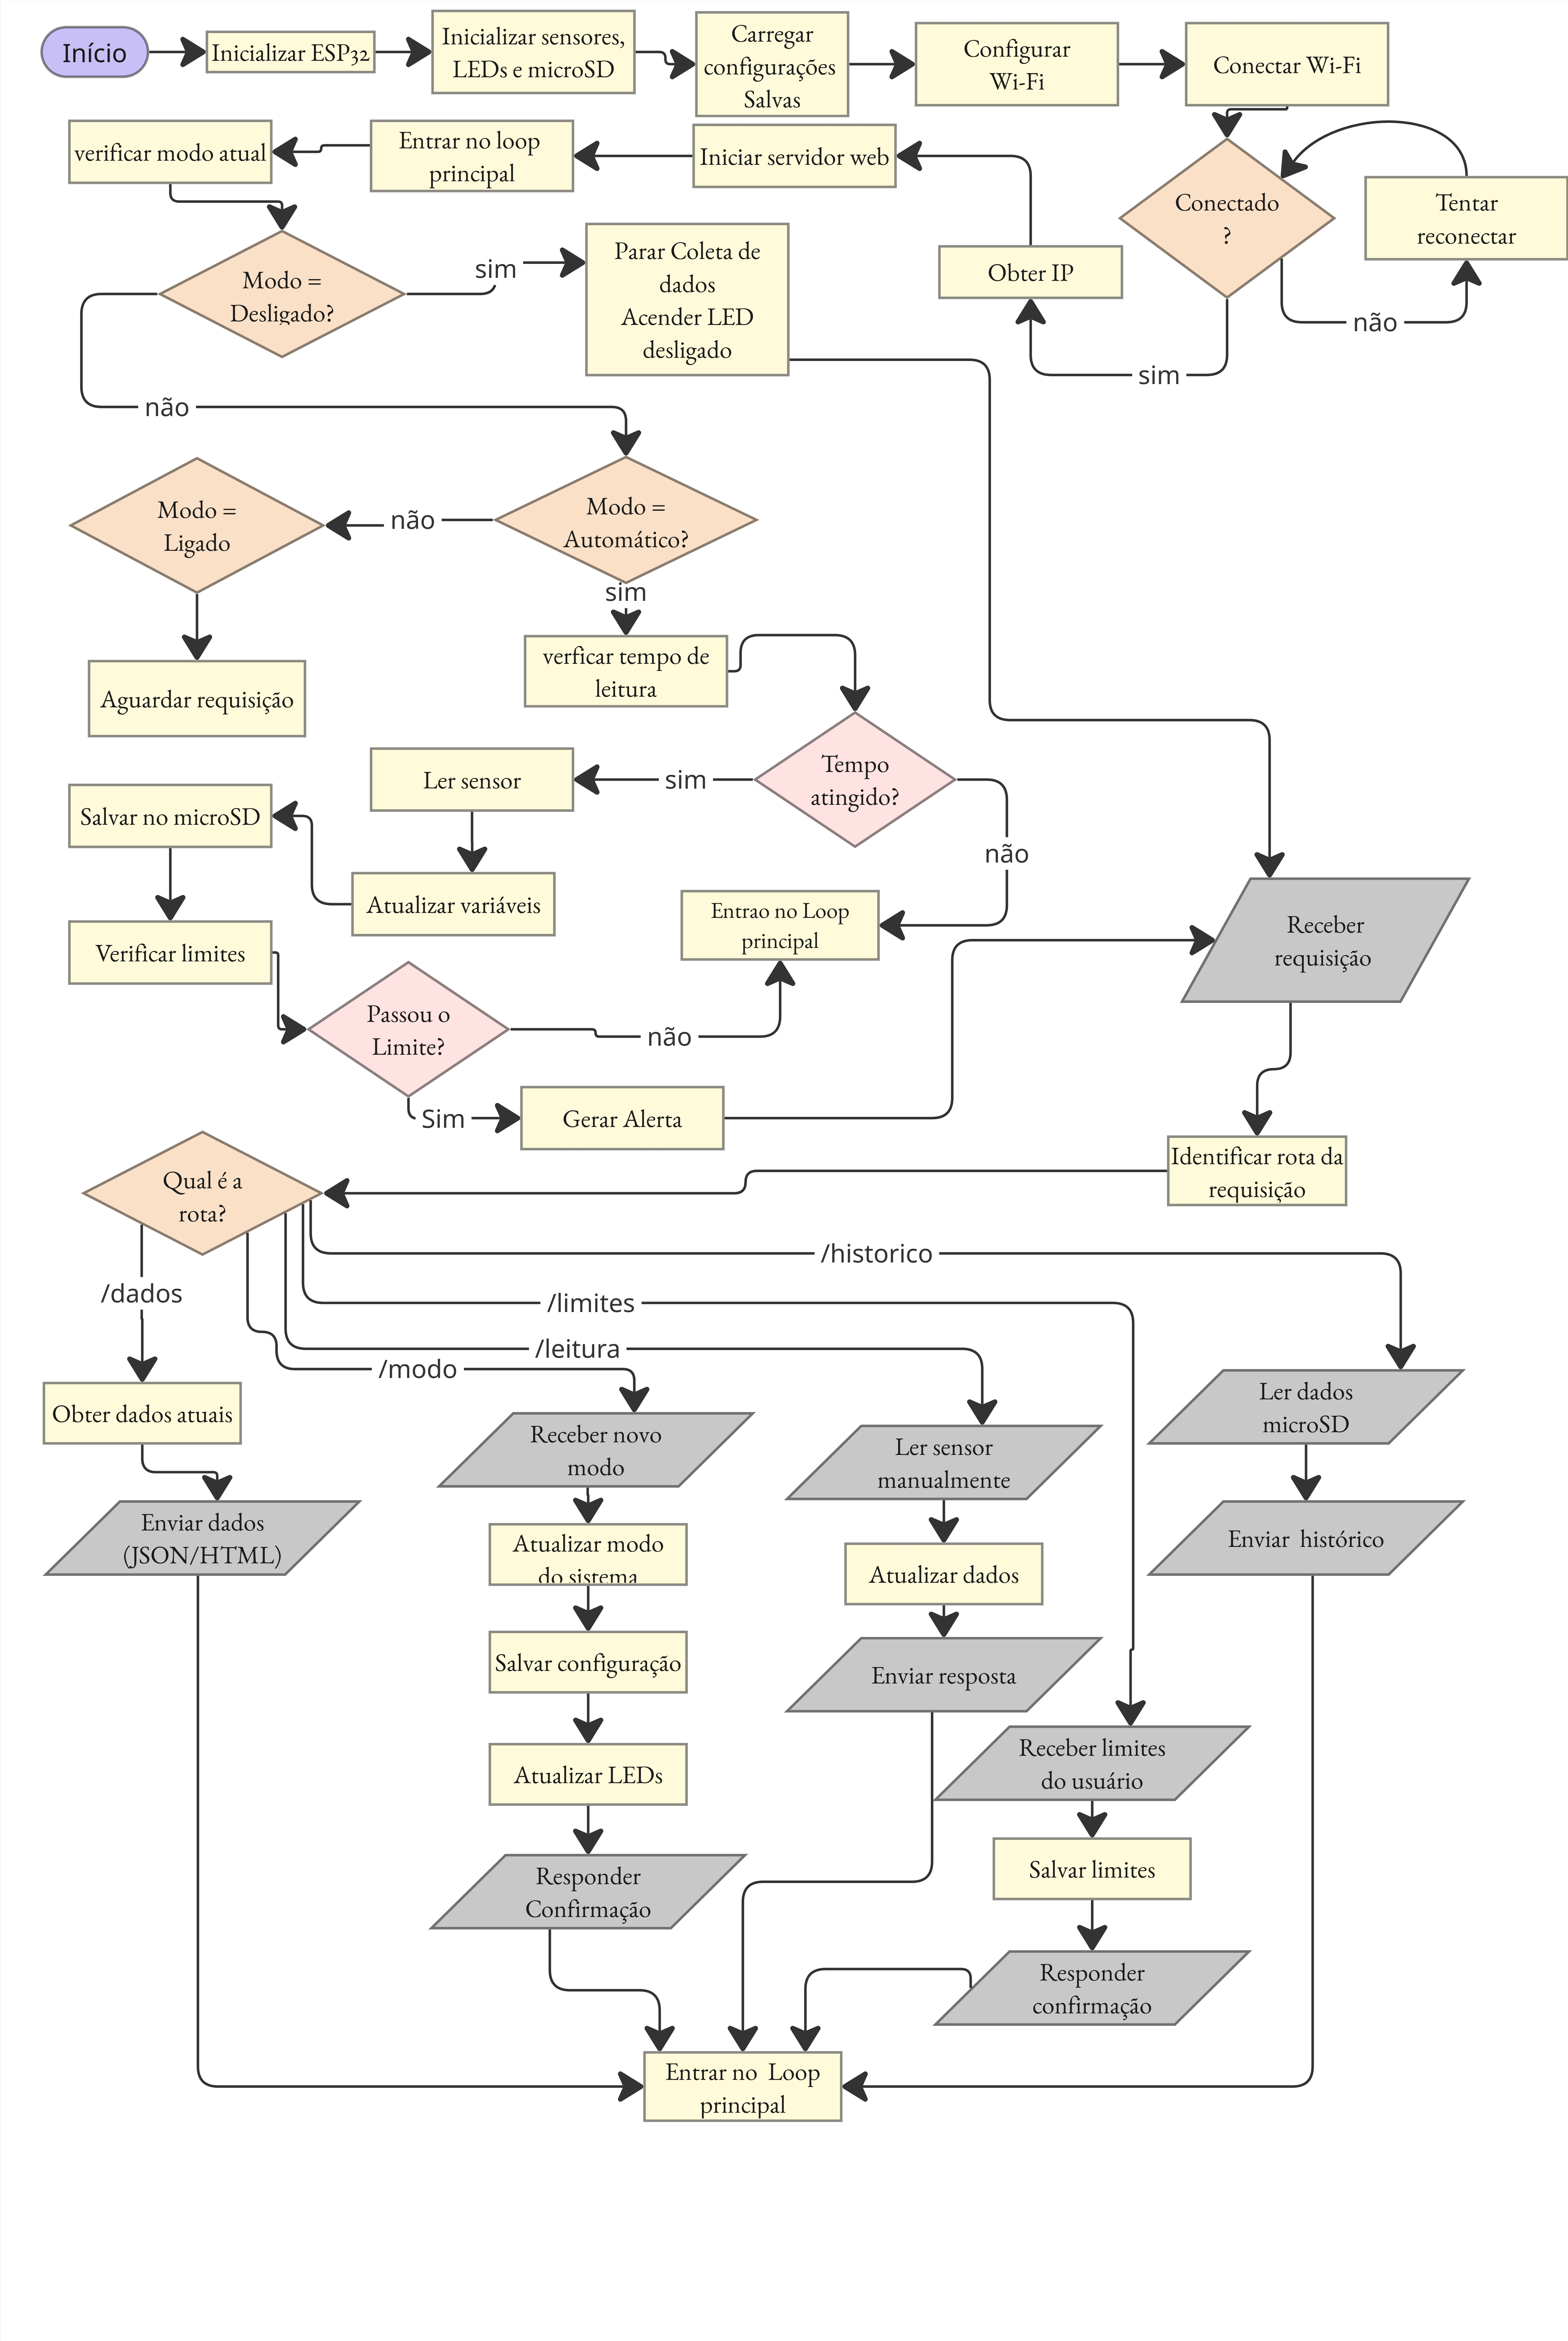
\includegraphics[width=0.8\textwidth]{img_arquivo/FluxoSoft.png} 
    \caption{Fluxograma de operação do software no ESP32}
    \label{fig:fluxograma_software}
\end{figure}

Com o intuito de nortear a execução das tarefas e garantir a eficiência dos processos, desenvolveu-se o fluxograma de software apresentado acima (Figura \ref{fig:fluxograma_software}). O diagrama detalha as etapas lógicas e as tomadas de decisão que compõem a arquitetura do sistema, demonstrando como ele alterna entre o modo automático de leitura e a escuta ativa de requisições HTTP via Wi-Fi.

\section{Protótipo de Interface}
\begin{figure}[H]
    \centering
    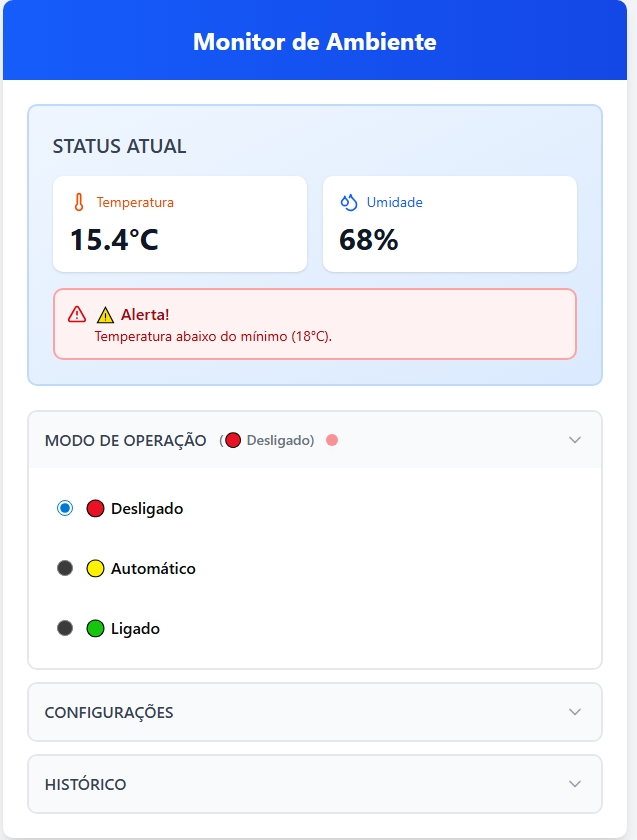
\includegraphics[width=0.5\textwidth]{img_arquivo/Prototipo_Interface.png} 
    \caption{Protótipo de Interface}
    \label{fig:prototipo_interface}
\end{figure}
\newpage



\section{Diagrama de Blocos}



\begin{figure}[H]
    \centering
    
\includegraphics[width=\textwidth]{LaTeX/img_arquivo/DiagramaDeBlocos.png}
    
    \caption{Diagrama de Blocos do Sistema de Monitoramento de temperatura e umidade em ESP32 DevKit}
    \label{fig:diagramaDeBlocos}
\end{figure}

\subsection*{Descrição do Diagrama}

O diagrama ilustra a arquitetura completa do sistema de monitoramento de temperaturae umidade do ambiente. O núcleo é o ESP32 DevKit, que recebe alimentação de 5V via USB e distribui internamente a referência de 3,3V para os periféricos. O Sensor AHT20 (temperatura e umidade) comunica-se com o ESP32 pelo barramento I²C (SDA/SCL). Os dados são armazenados localmente em um Módulo Micro SD via barramento SPI (MOSI, MISO, SCK, CS), que possui um level shifter integrado para adequação dos níveis de tensão. O ESP32 também publica as leituras em um Dashboard IoT acessível remotamente por Wi-Fi, utilizando protocolo HTTP com payload em JSON. Por fim, três LEDs controlados por GPIO indicam o estado operacional: verde (ligado), amarelo (automático) e vermelho (desligado/falha).

\newpage

\section{Modelagem do Circuito}

\begin{figure}[H]
    \centering
    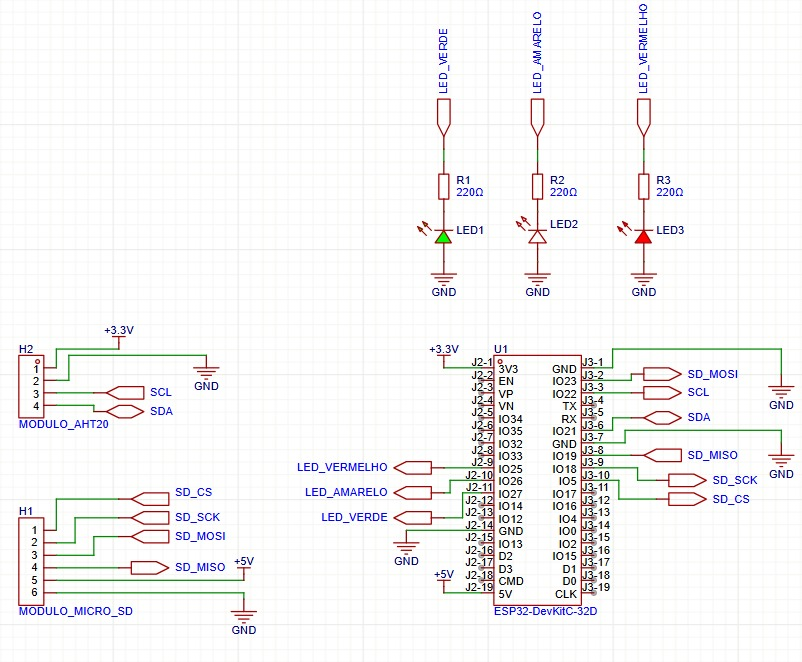
\includegraphics[width=1.0\textwidth]{img_arquivo/Esquematico.png} 
    \caption{Esquemático de Hardware}
    \label{fig:modelagem_de_circuitos}
\end{figure}

O diagrama elétrico detalha as conexões físicas entre o microcontrolador ESP32 e os periféricos do sistema. Nele, destaca-se a integração do sensor AHT20 via barramento I2C e a interface do módulo microSD via protocolo SPI. Além disso, o esquema apresenta o circuito de sinalização visual, composto por três LEDs (Verde, Amarelo e Vermelho) equipados com resistores de 220 $\Omega$ para garantir a proteção das portas lógicas do chip
\newpage

\section{Descrição de Hardware}
\input{Seções/Descricao de Hardware.tex}
\newpage

\section{Descricao de Alto nível}
\subsection{Subsistema de Alimentação e Regulação}
Este subsistema gerencia a conversão e distribuição de energia para garantir que cada componente opere dentro de sua faixa de tensão nominal, prevenindo danos ao hardware.

\begin{itemize}
    \item \textbf{Entrada de Energia}: O sistema recebe alimentação de 5V via porta Micro-USB, conectada diretamente ao computador ou fonte externa.
    \item \textbf{Regulação de Tensão (LDO)}: A placa DevKit utiliza um regulador de baixa queda (\textit{Low-Dropout} - LDO) para converter os 5V da entrada em 3,3V estáveis, necessários para o funcionamento do chip ESP32 e do sensor AHT20.
    \item \textbf{Barramento de 5V}: Este barramento alimenta o módulo de cartão SD, que por sua vez possui regulação própria e \textit{level shifters} internos para garantir a integridade dos sinais lógicos.
\end{itemize}

\subsection{Subsistema de Sensoriamento e Armazenamento}
Responsável por ler as informações do ambiente e salvá-las fisicamente.

\begin{itemize}
    \item \textbf{Sensor}: O AHT20 mede temperatura e umidade usando o protocolo I2C.
    \item \textbf{Gravação}: As leituras são salvas no cartão SD em arquivos \texttt{.csv} via protocolo SPI, garantindo que os dados fiquem guardados mesmo sem internet.
\end{itemize}

\subsection{Subsistema de Interface e Atuação}
Proporciona ao usuário uma visualização imediata do status operacional do dispositivo através de sinalizações luminosas.

\begin{itemize}
    \item \textbf{Sinalização Visual}: Três LEDs (Verde, Amarelo e Vermelho) compõem a interface física, permitindo identificar visualmente os estados de operação do hardware, estes leds funcionarão como: VERDE (ESTADO LIGADO), AMARELO (ESTADO AUTOMÁTICO), VERMELHO (ESTADO DESLIGADO)
    \item \textbf{Proteção Física}: Resistores limitadores de corrente são empregados em série com os LEDs, protegendo as saídas digitais do microcontrolador contra drenagem excessiva de corrente.
\end{itemize}

\subsection{Subsistema de Comunicação e Arquitetura de Software}
Este bloco gerencia a conectividade sem fio e a entrega da interface de usuário, permitindo o monitoramento remoto e a configuração do dispositivo em tempo real.

\begin{itemize}
    \item \textbf{Conectividade Wi-Fi}: O microcontrolador opera nos modos \textit{Station} (conectado a uma rede local) ou \textit{Access Point} (criando sua própria rede para configuração inicial), utilizando a pilha TCP/IP nativa do ESP32.
    \item \textbf{Servidor Web Assíncrono}: Utiliza-se a biblioteca \texttt{ESPAsyncWebServer} para processar requisições HTTP de forma não bloqueante. Isso garante que a entrega das páginas do site não interrompa as tarefas críticas, como a leitura do sensor AHT20 ou a escrita de logs no cartão SD.
    \item \textbf{Gerenciamento de Arquivos (LittleFS)}: Os arquivos de \textit{front-end} (HTML, CSS e JavaScript) são armazenados em uma partição da memória flash do microcontrolador organizada pelo sistema de arquivos LittleFS. Essa abordagem separa a lógica de controle (C++) da interface visual, otimizando o uso da memória RAM.
    \item \textbf{Interatividade (JSON e AJAX)}: A troca de dados entre o hardware e o navegador ocorre via pacotes JSON. Através de requisições assíncronas (AJAX), o site atualiza os valores de temperatura e umidade na tela automaticamente, eliminando a necessidade de recarregar a página pelo usuário.
\end{itemize}

\newpage

\section{Descrição de Firmware}
O firmware será desenvolvido em C++ para o ESP32, utilizando uma lógica assíncrona. Isso permite que o processador cuide da leitura dos sensores e do controle dos LEDs ao mesmo tempo em que mantém o servidor web funcionando, sem que uma tarefa trave a outra. A estrutura principal será uma máquina de estados, que define como o hardware deve se comportar em cada modo (Desligado, Automático ou Ligado).

\subsection{Sequência de Boot e Inicialização}
Assim que o sistema é ligado, o firmware executa os preparativos básicos para operar:
\begin{itemize}
    \item \textbf{Setup de Hardware:} O código inicia a comunicação I2C com o sensor AHT20 e a comunicação SPI com o módulo de cartão microSD
    \item \textbf{Conexão Wi-Fi:} O ESP32 busca a rede configurada e, após conectar, inicia o servidor web na porta 80 para permitir o acesso pela interface
\end{itemize}

\subsection{Ciclo de Execução e Máquina de Estados}
No laço principal do código, o firmware monitora as variáveis de estado e o tempo:
\begin{itemize}
    \item \textbf{Seleção de Modo:} O sistema verifica qual modo está ativo. No "Automático", ele faz leituras periódicas; no "Ligado", fica pronto para comandos; e no "Desligado", interrompe as leituras e acende o LED vermelho
    \item \textbf{Lógica de Sensoriamento:} O firmware lê o sinal do sensor e o converte para valores reais de temperatura ($^{\circ}C$) e umidade (\%)
    \item \textbf{Processamento de Alertas:} O código compara os dados com os limites definidos e, caso os valores saiam do normal, envia um sinal de alerta para a interface web
\end{itemize}

\subsection{Gerenciamento de Arquivos no microSD}
O sistema garante que as medições fiquem guardadas fisicamente:
\begin{itemize}
    \item \textbf{Rotina de Datalogger:} A cada nova coleta, o firmware abre o arquivo \texttt{dados.csv} no modo de anexo, salva a nova linha de informação e fecha o arquivo logo em seguida para garantir a segurança dos dados
    \item \textbf{Envio do Histórico:} Quando solicitado via site, o firmware lê as informações salvas no cartão e as envia para serem exibidas na tela do usuário
\end{itemize}

\subsection{Protocolo de Comunicação Web}
\markright{}
Esta parte cuida da troca de informações entre o código e o navegador:
\begin{itemize}
    \item \textbf{Tratamento de Requisições:} O servidor processa pedidos como a troca de modo (rota \texttt{/modo}) ou o envio dos dados atuais (rota \texttt{/dados}) em formato JSON
    \item \textbf{Sincronização de LEDs:} Sempre que o modo de operação muda pela interface, o firmware atualiza imediatamente o estado dos pinos GPIO, acendendo o LED correspondente (Verde, Amarelo ou Vermelho)
\end{itemize}
\newpage

\section{Bill of Materials}

A Tabela a seguir apresenta a lista de materiais (Bill of Materials - BOM) necessários para a implementação do sistema proposto, incluindo a descrição dos componentes, suas quantidades e os custos unitários estimados.
\begin{table}[h]
\centering
\vspace{0.2cm}
\begin{tabular}{|c|l|l|c|c|}
\hline
\textbf{ID} & \textbf{Componente} & \textbf{Descrição} & \textbf{Qntd} & \textbf{Preço Unit. (R\$)} \\ 
\hline
1  & ESP32 DevKitC V4     & MCU Wi-Fi WROOM-32D   & 1 & 45,00  \\ \hline
2  & Sensor AHT20         & Sensor Temp/Umid I2C  & 1 & 11,00  \\ \hline
3  & Módulo MicroSD       & SPI com level shifter & 1 & 9,90   \\ \hline
4  & Cartão microSD 8GB   & Classe 10, FAT32      & 1 & 15,00  \\ \hline
5  & LED Verde            & LED 5mm               & 1 & 0,50   \\ \hline
6  & LED Amarelo          & LED 5mm               & 1 & 0,50   \\ \hline
7  & LED Vermelho         & LED 5mm               & 1 & 0,50   \\ \hline
8  & Resistor 220$\Omega$ & 1/4W $\pm5\%$         & 3 & 0,25   \\ \hline
9  & Header fêmea         & Barra 2.54mm          & 1 & 3,00   \\ \hline
10 & Placa perfurada      & PCB universal 5x7cm   & 1 & 8,00   \\ \hline
\multicolumn{4}{|r|}{\textbf{Total Estimado (R\$)}} & \textbf{94,15} \\
\hline
\end{tabular}
\caption{Bill of Materials}
\end{table}

\end{document}